\documentclass[9pt]{article}
\usepackage{amsmath,amsfonts,amssymb,times}
\usepackage{graphicx,color,tikz,pgfplots}
\usepackage[paperwidth=13.5cm,paperheight=6.1cm,lmargin=0in,rmargin=0in,tmargin=0em,bmargin=0.in]{geometry}
\usepackage{bm}
\usetikzlibrary{arrows,shadings,shapes.arrows,decorations.pathreplacing,calc, positioning}
\usepgfplotslibrary{fillbetween}


\pagestyle{empty}
\pgfplotsset{compat=newest}
\definecolor{applered}{RGB}{255,8,0}
\definecolor{azure}{RGB}{0,127,255}
\definecolor{violet}{RGB}{159,0,255}

\pgfdeclareverticalshading{rainbow}{100bp}
{color(0bp)=(applered); color(25bp)=(red); color(40bp)=(yellow);
  color(47bp)=(green); color(51bp)=(cyan); color(60bp)=(blue);
  color(65bp)=(violet); color(100bp)=(violet)} 
                          
\newlength{\h}
\newlength{\rad}
\setlength{\h}{2cm}
\setlength{\rad}{1.5pt}

\def\seed{4}

\begin{document}
\centering
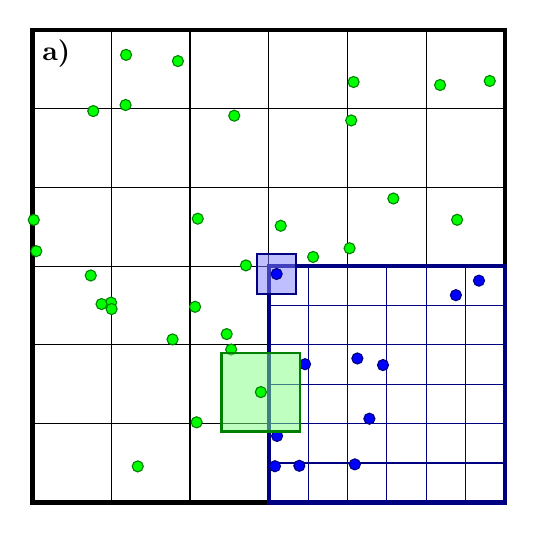
\begin{tikzpicture}[on grid]

  % Parent grid
  \draw[step=1cm, black, thin] (0,0) grid  (3\h,3\h); %defining grids
  \draw[black,ultra thick] (0,0) rectangle (3\h,3\h);%marking borders

  \pgfmathsetseed{\seed}
  \foreach \i in {1,...,40}
  \fill[fill=green, draw=green!50!black] (3*rnd*\h, 3*rnd*\h) circle(2pt);

  \draw[fill=white, densely dashed, draw=none, line width=3pt] (1.5\h, 0) rectangle (3\h, 1.5\h);
  
  % LEVEL 1 GRIDS
%  \draw[blue!50!black, ultra thick] (4,4) rectangle (8,8);%marking borders
  \draw[step=5mm, blue!50!black, thin] (1.5\h,0) grid (3\h,1.5\h);  %Nested grid 1
  \draw[blue!50!black, ultra thick] (1.5\h,0) rectangle (3\h,1.5\h);  %Nested grid 1
  \foreach \i in {1,...,10}
  \fill[fill=blue, draw=blue!50!black] (1.5\h + 1.5*rnd*\h, 1.5*rnd*\h) circle(2pt);

  % Blue particle with box
  \node[fill opacity=0.5, draw=blue!50!black, thick, fill=blue!50!white, minimum width=0.25\h, minimum height=0.25*\h, inner sep=0pt] at (1.55*\h, 1.45*\h) {};
  \fill[fill=blue, draw=blue!50!black] (1.55\h, 1.45\h) circle(2pt);

  % Green particle with box
  \node[fill opacity=0.5, draw=green!50!black, thick, fill=green!50!white, minimum width=0.5\h, minimum height=0.5*\h, inner sep=0pt] at (1.45\h, 0.7\h) {};
  \fill[fill=green, draw=green!50!black] (1.45\h, 0.7\h) circle(2pt);

  \node[anchor = north west] at (0\h, 3\h) {\bfseries a)};
\end{tikzpicture}
\hfill
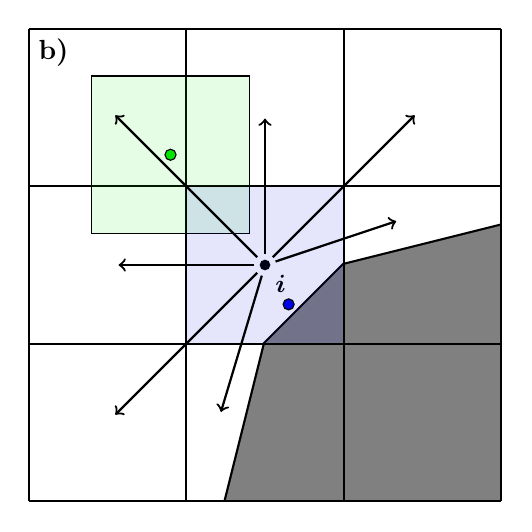
\begin{tikzpicture}[
    gridstyle/.style={thick,black},
    nodeCenterStyle/.style={thick,black,fill},
    surfaceStyle/.style={ultra thick,black},
    surfaceFill/.style={},
    phiStyle/.style={font=\small,anchor=south},
    redistStyle/.style={thick, black, ->, shorten >=4pt, shorten <=4pt}]

  %EB
  \path[name path=baseline] (1.5\h,0) -- (3\h,0);
  \draw[surfaceStyle,name path=surface] (1.25\h, 0) -- (1.5\h,\h) -- (2\h,1.5\h) -- (3\h,1.75\h);
  \tikzfillbetween[of=surface and baseline,on layer=,every segment/.style={surfaceFill}] {black!50!white};

  %% Grids and nodes
  \draw[step=\h,gridstyle] (0,0) grid (3\h,3\h);
  \draw[nodeCenterStyle] (1.5\h, 1.5\h) circle(\rad) node[phiStyle, below right] {$\bm{i}$};

  % Particles in regular and cut cells
  \draw[fill=green!90!black, fill opacity=0.1] (0.4\h, 1.7\h) rectangle ++(\h,\h);
  \draw[fill=blue!90!black, fill opacity=0.1] (1.\h, 1.\h) rectangle ++(\h,\h);
  
  \fill[fill=green!90!black, draw=black] (0.9\h, 2.2\h) circle(2pt);
  \fill[fill=blue!90!black, draw=black] (1.65\h, 1.25\h) circle(2pt);

  % Redistribution arrows
  \draw[redistStyle] (1.5\h, 1.5\h) -- (0.5\h, 0.5\h);
  \draw[redistStyle] (1.5\h, 1.5\h) -- (0.5\h, 1.5\h);
  \draw[redistStyle] (1.5\h, 1.5\h) -- (0.5\h, 2.5\h);
  \draw[redistStyle] (1.5\h, 1.5\h) -- (1.2\h, 0.5\h);
  \draw[redistStyle] (1.5\h, 1.5\h) -- (1.5\h, 2.5\h);
  \draw[redistStyle] (1.5\h, 1.5\h) -- (2.4\h, 1.8\h);
  \draw[redistStyle] (1.5\h, 1.5\h) -- (2.5\h, 2.5\h);

  \node[anchor = north west] at (0\h, 3\h) {\bfseries b)};
\end{tikzpicture}
\end{document}
